\documentclass[10pt,letterpaper,oneside]{article}
\usepackage[utf8]{inputenc}
\usepackage{amsmath}
\usepackage{amsfonts}
\usepackage{amssymb}
\usepackage{graphicx}
\usepackage{float}
\begin{document}

\large{Portfolio Balancer-- Outline}
\section{Formulas}

The total portfolio application is a constraint. In dimensionless form this looks like
\begin{equation}
1=\sum_{i}|\delta_i|
\end{equation}
This is the equation of a hyper octahedron
\begin{figure}[H]
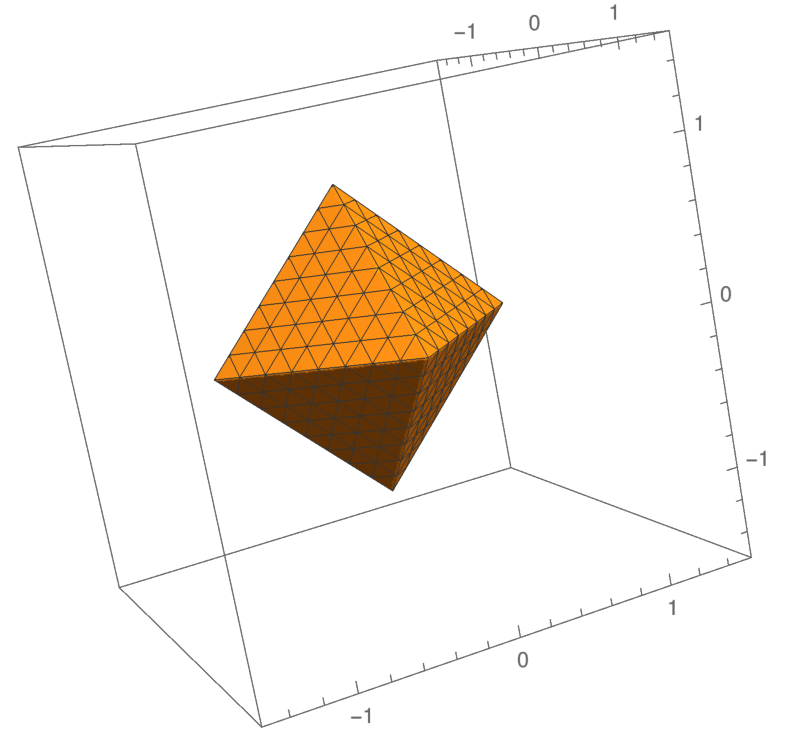
\includegraphics[scale=1]{tetra}
\caption{Portfolio constraint surface in three dimensions. The various faces correspond to longing or shorting different stocks.}
\end{figure}

The absolute value is there to account for shorts. A better parametrization is needed.
\begin{equation}
C_1:\,\,\,1=\sum_{i}x_i^2
\end{equation}
This is the equation for a hypersphere. So we can use the following parametrization if needed
\begin{equation}
\begin{split}
x_1&=\cos{(\theta_1)}\\
x_2&=\sin{(\theta_1)}\cos{(\theta_2)}\\
x_3&=\sin{(\theta_1)}\sin{(\theta_2)}\cos{(\theta_3)}\\
x_4&=...
\end{split}
\end{equation}
This implements the constraint automatically. Though it may be too hard to use.

We also have the $\beta$ of the portfolio
\begin{equation}
\beta_{p}=\sum_{i}\text{sign}{(x_i)}x_i^2 \beta_i=\vec{\delta}\cdot \vec{\beta}
\end{equation}
and the expected  return
\begin{equation}
r_{p}=\sum_{i}\text{sign}{(x_i)}x_i^2 r_i=\vec{\delta}\cdot \vec{r}
\end{equation}
the active return
\begin{equation}
\alpha_{p}=\sum_{i}\text{sign}{(x_i)}x_i^2 \alpha_i=\vec{\delta}\cdot \vec{\alpha}
\end{equation}
The variance

\begin{equation}
\sigma_{p}^2=\sum_{i,j}\delta_i \text{Cov}(r_i,r_j)\delta_j=\vec{\delta}' \text{Cov}(\vec{r},\vec{r})\vec{\delta}
\end{equation}


We then have for the sharpe ratio

\begin{equation}
S_p=\frac{\vec{\delta}\cdot \vec{r}}{\sqrt{\vec{\delta}' \text{Cov}(\vec{r},\vec{r})\vec{\delta}}}
\end{equation}

\subsection{Minimizing the Volatility}
Supposing we want to minimize the volatility $\sigma_p^2$ for a portfolio composed of about a hundred stocks. This not a clearly trivial problem because then this hyper octahedra will have $2^{100}$ faces. So one cannot search all of them. This is a constrained optimization problem

\subsection{Attempt 1}
\begin{equation}
\mathcal{L}=\delta_i C_{i j} \delta_j-\lambda \left(\sum_{i}|\delta_i|-1\right)
\end{equation}

Then we have the equations
\begin{equation}\label{crit}
0=2 C_{i j}\delta_j-\lambda \,\,\text{sign}(\delta_i)
\end{equation}

multiplying by $\delta_i$ and summing gives
\begin{equation}
\frac{\lambda}{2}=\delta_i C_{i j} \delta_j
\end{equation}
giving us the value of the lagrange multiplier. we can then solve (\ref{crit}). Again this is still non trivial because the sign function is not amenable to numerical root finding methods and there are too many faces too brute force search. To get a better idea, we can consider the figure in two dimensions.

\begin{figure}[H]
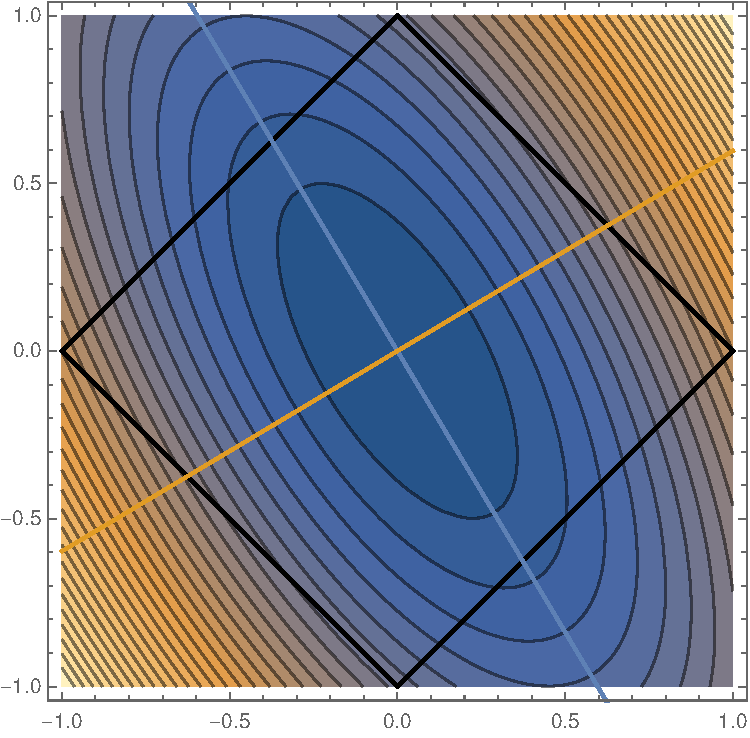
\includegraphics[scale=1]{concept}
\caption{Contour of the volatility with constraint imposed. Lines shown are parallel to the eigen vectors of the covariance matrix}
\end{figure}

The physical intution gained from the figure is that the eigenvector with the smallest eigenvalue points at the face where the minimum lies. If the off diagonal correlations are exactly zero then the eigenvectors point at the corners so then this wouldn't work. However, then even numerical errors would break the symmety. Maybe check for this case as an edge case in the implementation. Nevertheless Supposing this is true we should have
\begin{equation}
\text{sign}(\delta^{min})=\text{sign}\left(\frac{e^{min}}{||e^{min}||_1}\right)
\end{equation}
because both quantities are specified by the face we are on. And $e^{min}$ is the eigenvector of C with the lowest eigenvalue. BTW all eigenvectors of C should be real and positive. otherwise one could construct a portfolio with negative variance. Then we have the equation for $\delta$
\begin{equation}
C_{i j}\delta_j-\delta_k C_{k l} \delta_l\,\,\text{sign}\left(e^{min}_i\right)=0
\end{equation}
This is easier to solve, because now we don't have to worry about the non analyticity of the sign function and the many faces. This can be solved for instance by newtons method.

\subsection{Attempt 2}
We use the intuition from the last attempt. That is the lowest weight eigenvector points at the face where the constrained minimum is. Once this face is specified, we can then use gradient descent in order to find the minmum on that plane. Let $\hat{n}$, be the normalized eigenvector to the specified face. Then we have the recursion
\begin{equation}
\delta^{n+1}=\delta^{n}-2 \alpha\left(C \vec{\delta}^n-(\hat{n}C \vec{\delta}^n)\hat{n}\right)
\end{equation}
The second term in the brackets there assures that we stay on the same plane and $\alpha$ is the learning rate, which we get to specify. In our two dimensional example, this strategy does quite well.

\begin{figure}[H]
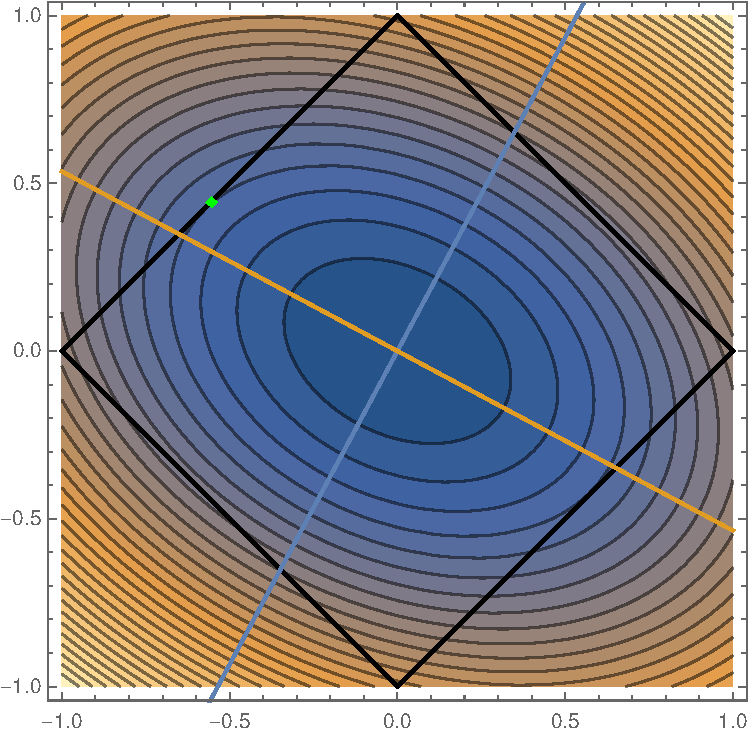
\includegraphics[scale=1]{Mined}
\caption{Constrained minimization of the volitility. The green diamond, marks the location of the constrained minimum of the volitility. The parameters used here are: $\sigma_x^2=0.8$, $\sigma_y^2=1.2$,$\text{Cov}(x,y)=0.3$, The minimized volitilty is $\sigma_p^2=0.33$. For comparison the lowest eigenvalue of the covariance matrix is $\lambda_{min}=0.65$. So we get a considerable decrease in the volitility this way.}
\end{figure}

generally, there will be two solutions here. We can break this tie by factoring in the behavior of the market. If there is a bull market, we choose the solution that has positive $\beta\cdot \delta$. If there is a bear market, we choose the solution that has negative $\beta\cdot \delta$

\section{Maximizing the Sharpe ratio}
\subsection{Attempt 1}
The Sharpe ratio is given by
\begin{equation}
S=\frac{\delta_i r_i}{\sqrt{\delta_i C_{ij}\delta_j}}
\end{equation}
This has the gradient
\begin{equation}\label{grad}
\partial_{\delta_i}S=\frac{r_i \sqrt{\delta_i C_{ij}\delta_j}-(\delta_k r_k)\frac{C_{ij}\delta_j}{\sqrt{\delta_i C_{ij}\delta_j}}}{\delta_i C_{ij}\delta_j}
\end{equation}

we notice that 
\begin{equation}
\delta_i \partial_{\delta_i}S=0
\end{equation}
Since the gradient is perpendicular to the level curves, and since $\delta $ is a vector with it's tail at the origin, the level curves of S are lines stemming from the orgin. From here, we can do gradient descent on the unit \emph{sphere}, rather than octahedron, using (\ref{grad}). Then we can renormalize with the $l_1$ norm to get the final porfolio allocation.

\subsection{Attempt 2}
\begin{equation}
\begin{split}
S&=\frac{\delta_i r_i}{\sqrt{\delta_i C_{ij}\delta_j}}\\
&=\frac{e_i \bar{r}_i}{\sum_j \lambda_j e_j^2}\\
&=\frac{\sqrt{\lambda_i}e_i \bar{r}_i/\sqrt{\lambda_i}}{\sum_j \lambda_j e_j^2}\\
\end{split}
\end{equation}
Therefore, this vector $\sqrt{\lambda_i}e_i$ should be parallel to $\bar{r}_i/\sqrt{\lambda_i}$ in order to maximize the sharpe ratio
so we have
\begin{equation}
e_i=\frac{\bar{r}_i}{\lambda_i}
\end{equation}
so
\begin{equation}
O_{ij}\delta_j=\sum_j \frac{1}{\lambda_i}O_{i j}r_j
\end{equation}
Then
\begin{equation}
\delta^{max}_{i}=\sum_{k l}O_{i k}\frac{1}{\lambda_k}O_{k l}r_l
\end{equation}
We recognize that sum
\begin{equation}
\delta^{\max}_{i}=C^{-1}_{ij}r_j
\end{equation}
This needs to be normalize wrt the l1 norm.
So then the max Sharpe ratio achievable is
\begin{equation}
S_{max}=\sqrt{r_i C^{-1}_{ij}r_j}
\end{equation}
\section{Risk weighted beta}
Depending on whether we are in a bull or bear phase of the market we want to maximize the movement of our portfolio, so max(min)imizing $\beta$. However, beta is maximized by just projecting onto the axis with the highest beta. Therefore, we should introduce a risk weighted beta: $\mathcal{B}=\frac{\beta \cdot \delta}{\sqrt{\delta_i C_{ij}\delta_j}}$. This quantity is minimized or maximized according to the same proceudre as the sharpe ratio.

\begin{equation}
\mathcal{B}_{max}=\sqrt{\beta_i C^{-1}_{ij}\beta_j}
\end{equation}
and
\begin{equation}
\delta=\pm \frac{C^{-1}_{ij}\beta_j}{l1(C^{-1}_{ij}\beta_j)}
\end{equation}

\section{Strategy}
The basic strategy we will implement:
\begin{itemize}
\item if one year moving average is below the 2 month moving average by one sigma, minimize the risk weighted beta. 
\item if one year moving average is above the 2 month moving average by one sigma maximize the risk weighted beta.
\item in the one sigma range around the 1 year moving average, construct a market neutral portfolio that can take advantage of the active returns.
\end{itemize}





\end{document}